\documentclass[aspectratio=169]{beamer} % O parâmetro aspectratio com valar 16:9 deixa o slide em widescreen

\usepackage[brazil]{babel}
\usepackage[utf8]{inputenc}
\usepackage[T1]{fontenc}
\usepackage{listings}
\usepackage{textcomp}

\usetheme{Madrid}
\setbeamertemplate{navigation symbols}{}

\title[Eletrônica]{Eletrônica}

\author[Diego S. C. Nascimento]{Diego Silveira Costa Nascimento}

\institute[IFRN]{
Instituto Federal de Educação, Ciência e Tecnologia do Rio Grande do Norte\\
diego.nascimento@ifrn.edu.br
}

\date[\today]{\today}

\begin{document}

\begin{frame}[plain]
	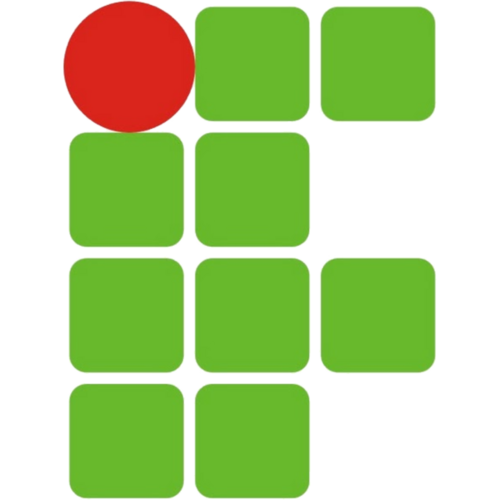
\includegraphics[scale=0.2]{img/IFRN}
	\titlepage
\end{frame}

\logo{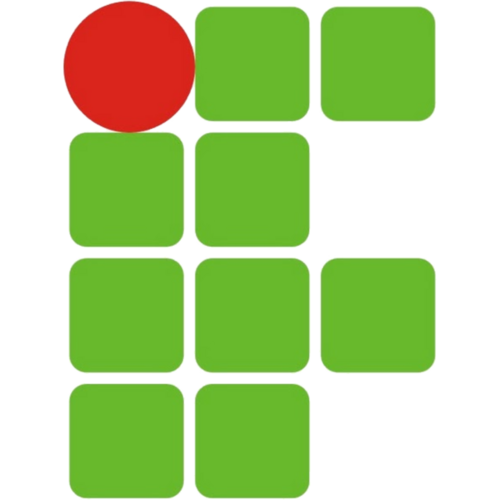
\includegraphics[scale=0.1]{img/IFRN}}

\begin{frame}
	\frametitle{Eletricidade}
	
	\begin{itemize}
		\item É uma forma de energia resultante do movimento de partículas carregadas;
		\item Essa energia pode ser gerada por fontes naturais ou artificiais;
		\item É essencial para o funcionamento de dispositivos e sistemas no mundo moderno;
		\item Pode ser classificada como:
		\begin{itemize}
			\item Estática; ou
			\item Dinâmica.
		\end{itemize}
	\end{itemize}
\end{frame}

\begin{frame}
	\frametitle{Tensão elétrica}
	
	\begin{itemize}
		\item É a força que impulsiona as cargas elétricas através de um condutor;
		\item Representa a diferença de energia elétrica entre dois pontos de um circuito;
		\item Para que a corrente elétrica flua, deve existir uma \structure{diferença de potencial} entre esses pontos, o que gera um movimento de elétrons; e
		\item A unidade de medida da tensão elétrica é o Volt $(V)$.
	\end{itemize}
\end{frame}

\begin{frame}
	\frametitle{Corrente elétrica}
	
	\begin{itemize}
		\item A corrente elétrica é o fluxo de cargas elétricas (elétrons) através de um material condutor;
		\item A unidade de medida da corrente elétrica é o Ampère $(A)$;
		\item Tipos de corrente:
		\begin{itemize}
			\item Corrente contínua; ou
			\item Corrente alternada.
		\end{itemize}
	\end{itemize}
\end{frame}

\begin{frame}
	\frametitle{Corrente contínua vs Corrente alternada}
	
	\begin{center}
		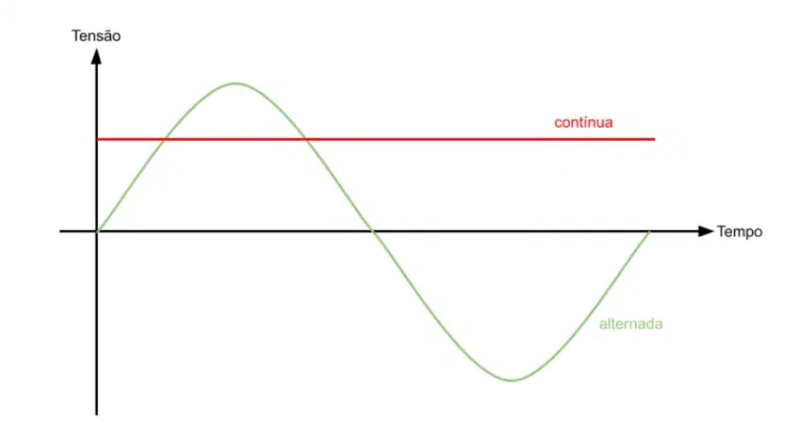
\includegraphics[scale=0.5]{img/cc-ca}
	\end{center}	
\end{frame}


\begin{frame}
	\frametitle{Resistência elétrica}
	
	\begin{itemize}
		\item É a oposição ao fluxo de corrente elétrica dentro de um material;
		\item Ela é gerada pelas interações entre as partículas do material e as cargas elétricas, que dificultam o movimento das cargas;
		\item A unidade de medida da resistência elétrica é o Ohm $(\Omega)$.
	\end{itemize}
\end{frame}

\end{document}